\documentclass[a4paper,12pt]{article}
%\usepackage[utf8]{inputenc}
\usepackage {fontspec} %,xunicode} %,xltxtra}
%	\setmainfont{Times New Roman}
\setmainfont[
Ligatures={TeX,Common},
PunctuationSpace=0,
Numbers={Proportional},
BoldFont = LibertinusSerif-Semibold.otf,
ItalicFont = LibertinusSerif-Italic.otf,
BoldItalicFont = LibertinusSerif-SemiboldItalic.otf,
BoldSlantedFont = LibertinusSerif-Semibold.otf,
SlantedFont    = LibertinusSerif-Regular.otf,
SlantedFeatures = {FakeSlant=0.25},
BoldSlantedFeatures = {FakeSlant=0.25},
SmallCapsFeatures = {FakeSlant=0},
]{LibertinusSerif-Regular.otf}

%% Trigger answers and notes. Package by Byron Ahn with edits by Craig Sailor
\usepackage[solution]{myProbSol} %   Optional arguments:
%                                               'solution': reveals solutions
%                                               'spaces': leaves whitespace corresponding to the size of the solutions (has no effect if you also pass 'solution')

\usepackage[margin={1in}]{geometry}

\usepackage[dvipsnames]{xcolor}
\usepackage[linkcolor=purple,citecolor=ForestGreen,colorlinks=true,urlcolor=purple,pagebackref=false]{hyperref}

\usepackage{natbib}
\bibpunct[:]{(}{)}{;}{a}{}{,}
\setlength{\bibsep}{0pt plus 0.3ex}
\usepackage{graphicx}
\usepackage{multicol}
\usepackage{amsmath}
\usepackage{expex} %Linguistics examples
\lingset{aboveexskip=0.2ex,belowexskip=0.8ex,aboveglftskip=-0.2ex,interpartskip=0.2ex,labelwidth=!6pt,belowpreambleskip=0.1ex} %, *=*?}
\newcommand\trace{\rule[-0.5ex]{0.5cm}{.4pt}}
\newcommand\denote[1]{$\llbracket$#1$\rrbracket$}
\newcommand\lra{$\leftrightarrow$}

\usepackage{mdwlist}  %
\usepackage[normalem]{ulem}
\usepackage{array} % >{\...} in tabulars
\setlength\parindent{0pt}
\usepackage{dashrule} %\hdashrule

\usepackage{lastpage}
\usepackage{fancyhdr}
\addtolength{\headheight}{2.5pt}
\pagestyle{fancy} %or fancyplain
\lhead{Morphology 2024-25 (UoE)}
\rhead{Word jigsaw}
\fancyfoot[C]{\thepage~of \pageref{LastPage}}
\fancypagestyle{plain}{%
\fancyhf{} % clear all header and footer fields
\fancyfoot[C]{Page \thepage~of \pageref{LastPage}} % except the center
\renewcommand{\headrulewidth}{0pt}
\renewcommand{\footrulewidth}{0pt}}

\newcommand\blue[1]{\textcolor{blue}{#1}}
\definecolor{edir}{RGB}{193,0,67}
\definecolor{edib}{RGB}{0,50,95}
\newcommand\ruler{{\centering \color{edir} \rule[-0.5em]{0.6\columnwidth}{0.4pt}\par}}

\renewcommand\root[1]{$\sqrt{\text{#1}}$}

\usepackage{pifont}
\newcommand{\cmark}{\ding{51}}% 52
\newcommand{\xmark}{\ding{55}}%
\newcommand{\hand}{\ding{43}}

\newcommand\gsc[1]{\textsc{\lowercase{#1}}} %for glossing in small caps - comment out to return to caps

\makeatletter %Allow superscript ^ and subscript _
\catcode`_=\active%
\gdef_#1{\ensuremath{{}\sb{#1}}}%
\catcode`^=\active%
\gdef^#1{\ensuremath{{}\sp{#1}}}%
\makeatother

\title{Word jigsaw}
\date{Morphology 2024-25}
\author{}

\begin{document}

In this activity we want to understand some of the potential weaknesses in our syntactic approach to morphology. There are a few small jigsaw ``pieces'' here for you to choose from. Each group will most likely only have time to focus on one or two of them.


\begin{answer}
{
These activities all challenge the assumption that morphology can be seen as the combination of morphemes. In one way or another, they all try to point to the existence of the word (or the stem) as an independent element that a theory of morphology needs to have.
}
\end{answer}

\section{Morphophonology: Anythin'}

The following informal pronunciations are common in many varieties of English, where the final /g/ is velarised into an [ŋ]:
\pex \label{ex:ing}
    \a \emph{laughing} $\rightarrow$ \emph{laughin'}
    \a \emph{jumping} $\rightarrow$ \emph{jumpin'}
\xe
\pex
    \a \emph{nothing} $\rightarrow$ \emph{nothin'}
    \a \emph{something} $\rightarrow$ \emph{somethin'}
\xe

\bigskip
It's been suggested that not all quantifiers can undergo the same reduction as in~(\lastx):
\pex
    \a \emph{everything} $\rightarrow$ *\emph{everythin'}
    \a \emph{anything} $\rightarrow$ *\emph{anythin'}
\xe

\paragraph{Q1} What are your intuitions? Is this the case for the varieties you speak as well?

\begin{answer}
{Definitely not all varieties! And it's actually unclear how robust these claims are.}
\end{answer}

\paragraph{Q2} Assume for the sake of the argument that the reductions in~(\lastx) really aren't possible. What challenge could this pose for our theory?
\begin{answer}
{
The idea here is that~(\lastx) might indicate storage of an entire word, rather than a compound made up of two morphemes. Suppose that~(\ref{ex:ing}) shows us that progressive -\emph{ing} can be reduced and that~(\lastx) shows us that \emph{thing} can be reduced in a compound. Then why can't we get~(\lastx)? In that case, we might not be talking about \emph{every+thing} but about one word \emph{everything}.\\
Now, there are a number of things we could say. Perhaps this has to do with the phonology of the first element of the compound. Perhaps it's telling that just \emph{thing} on its own cannot usually be reduced to \emph{thin'}. These are some of the possible explanations we could look for, but the point here was less about the analysis, and more about what a challenge to a morpheme-based approach could look like.
}
\end{answer}


\section{Allomorphy: Suppletion across words}

Our investigation of suppletion looked at examples such as the following, where the form (allomorph) of a \uline{Tense} affix depends on the \fbox{Perf} morpheme/feature:

\begin{multicols}{2}
\pex \label{ex:perf-agr-past}
    \a \begingl
        \gla am-\=a-\underline{ba}-\textbf{m}//
        \glb \root{am}-\gsc{TH}-\underline{Past}-\textbf{\gsc{1SG}}//
        \glft `I loved'//
    \endgl

    \a \begingl
        \gla am-\=a-\fbox{ve}-\underline{ra}-\textbf{m}//
        \glb \root{am}-\gsc{TH}-\fbox{Perf}-\underline{Past}-\textbf{\gsc{1SG}}//
        \glft `I had loved'//
    \endgl
\xe
\end{multicols}

What about allomorphy not between affixes, but between ``words'' (phonological words)? The indefinite article in English is sensitive inwards to phonology. But there's reason to think that the article cliticises onto the following word, forming a phonological word with it:

\pex \label{ex:en-indef}
    \a   \emph{a dog}		 [əˈdɑg]
 	\a  \emph{an apple} [əˈnæpl̩]
\xe
% \ex
%   D[\textminus{}def] \lra $\begin{cases} 
% 	\emph{\text{ə}} & / \trace~ \#\text{C} \\
% 	\emph{\text{ən}} & / \trace ~ \#\text{V} \\
% 	\end{cases}$ 
% \xe

\paragraph{Q1} What would suppletion triggered between phonological words look like? Can you think of any examples from languages you're familiar with?
\begin{answer}
{The claim is that there are no such cases.}
\end{answer}

\paragraph{Q2} How would that be different from the choice of auxiliary in English, as in \emph{will be eaten}, \emph{has been eaten}, \emph{will have been being eaten}, and so on?
\begin{answer}
{We discussed evidence for these auxiliaries all being separate morphemes, i.e.~separate heads in a syntactic structure.}
\end{answer}

\paragraph{Q3} If none of these (or few of these) are really attested, what does that mean for our view of morphology?
\begin{answer}
{
In our view of morphology, there's no such thing as a morphological ``word'', but there are phonological words that are different from affixes. If suppletion is really about two morphemes in a structure looking at each other, then it shouldn't matter whether they're affixes or phonological words. But it looks like it does.
}
\end{answer}


\section{Morphosyntax: Romance paradigms}

Here's a typical paradigm for the present tense indicative verb `eat' in Galician:

\begin{tabular}{lll}
        & \gsc{SG} & \gsc{PL}\\\hline
    1 & com-o    & come-mos\\
    2 & come-s   & come-des\\
    3 & come    & come-n\\
\end{tabular}

Even without knowing much about the phonology of the language, we can identify one root \gsc{COME(R)} (with the infinitival \emph{r}) and basic stem \emph{com-}, alongside a few inflectional endings. This is a fairly regular verb. Those of you familiar with Romance languages might want to decompose the stem even further into a root and a theme vowel.

% \bigskip
% Here is the irregular verb `to be (in a current state)'; ignore the accent marks, which are purely orthographic:

% \begin{tabular}{lll}
%         & \gsc{SG} & \gsc{PL}\\\hline
%     1 & est-ou    & esta-mos\\
%     2 & est\'a-s   & esta-des\\
%     3 & est\'a   & est\'a-n\\
% \end{tabular}

% It looks like the stem is the same throughout the paradigm, with the slight exception of \gsc{1sg}. Assuming that agreement is somewhere on the T, I or Agr heads, we can express this as suppletion of that head when it has the relevant feature:
% \pex
%     \a \root{\gsc{estar}} \lra{} \emph{est} / \trace{} \gsc{1SG}
%     \a \root{\gsc{estar}} \lra{} \emph{esta} [elsewhere]
% \xe

\bigskip
Some verbs are irregular, regardless of theme vowel. Here is `to do':

\begin{tabular}{lll}
        & \gsc{SG} & \gsc{PL}\\\hline
    1 & fago    & facemos \\
    2 & fas   & facedes \\
    3 & fai    & fan \\
\end{tabular}

\paragraph{Q1} What would we need to say in order to account for the distribution of stems now? What does the allomorphy depend on?
\begin{answer}
{
We have at least two, maybe three or four different stems. One for \gsc{1SG} \emph{fag-}, one for \gsc{2PL, 3PL} \emph{fac(e)-}, and \emph{fa(i)-}.
We'd need to say that we have one allomorph in \gsc{1SG}, while the others don't form \emph{natural classes}. That is, we'd either need to say that we have \emph{fac(e)-} for all plural forms \textbf{except} 3rd person, or that we have it in \gsc{1PL} \textbf{and also} \gsc{2PL}.
}
\end{answer}

\bigskip
This pattern exists in many irregular verbs. Here's `go' as well:

\begin{tabular}{lll}
        & \gsc{SG} & \gsc{PL}\\\hline
    1 & vou    & imos \\
    2 & vas   & ides \\
    3 & vai    & van \\
\end{tabular}

\paragraph{Q2} Would we now need to apply the same solution as in Q1 to each and every irregular verb that behaves the same way? Is this a problem?
\begin{answer}
{
The idea here is that we could come up with some clunky list of allomorphs like in the proposed answer to Q1. But then we'd need to come up with the same kind of list for almost every irregular verb in and across languages, which indicates that we're missing a larger generalization.
}
\end{answer}


\bigskip
Many Romance languages show similar pattens. Here's `go' in Italian:

\begin{tabular}{lll}
    & \gsc{SG}  & \gsc{PL} \\\hline
     \gsc{1} &  vado   & andiamo  \\
     \gsc{2} & vai  & andate \\
     \gsc{3} & va   & vanno \\
\end{tabular}

\bigskip
And here's the conjugation for `come' in the Italian indicative and subjunctive moods.

\begin{tabular}{lll}
        & \gsc{IND} & \gsc{SBJ}\\\hline
    \gsc{1SG}   & vengo    &  venga\\
     \gsc{2SG}  & vieni    & venga  \\
     \gsc{3SG}  & biene    & venga\\ 
\end{tabular}

\paragraph{Q3} Has the problem gotten worse? In what ways?
\paragraph{Q4} How might this be a challenge for our current theory?
\begin{answer}
{
In other cases of allomorphy we could say that we don't need two verbs \emph{go} and \emph{went}, but one allomorph \emph{go} and one allomorph \emph{went} in the context of T[Past].\\
With these examples the listing of allomorphs wouldn't be as clean. Listing them all is possible, but very clunky, and not clearly better than talking about the stems in a paradigm as their own, non-morphemic objects. Discussion of these patterns sometimes calls them \emph{morphomes}(!).
}
\end{answer}

\section{Lexical processing: Whole-word lookup}
We've seen evidence that we decompose anything that looks like a suffix when we see it in written form, even if we're only exposed to it for 40ms. We also mentioned that there's a way to quantify the neural response associated with this decomposition by looking at \emph{transition probability} (\textbf{TP}): the TP of \emph{formid-able} is greater than that of \emph{tax-able}, because you're much more likely to go from \emph{formid} to \emph{-able} than from \emph{tax} to \emph{-able}.

TP is correlated with very early activation, between 150--200ms after seeing the word; this neural components is called the ``M170'' (``M'' for MEG and ``170'' for 170ms).

\bigskip
Other factors that researchers look at include the overall \emph{frequency} of the word.

\bigskip
In one MEG experiment, participants saw ``pseudo-affixed'' words like \emph{brother} and \emph{corner}. Here are some of the findings. Focus on the plot on the left: in shows the M170 as correlated with the frequency of the word (SF) and transition probability (TP), as well as another factor (base frequency, BF).

\paragraph{Q1} What does the M170 seem to be tracking here?


\begin{center}
    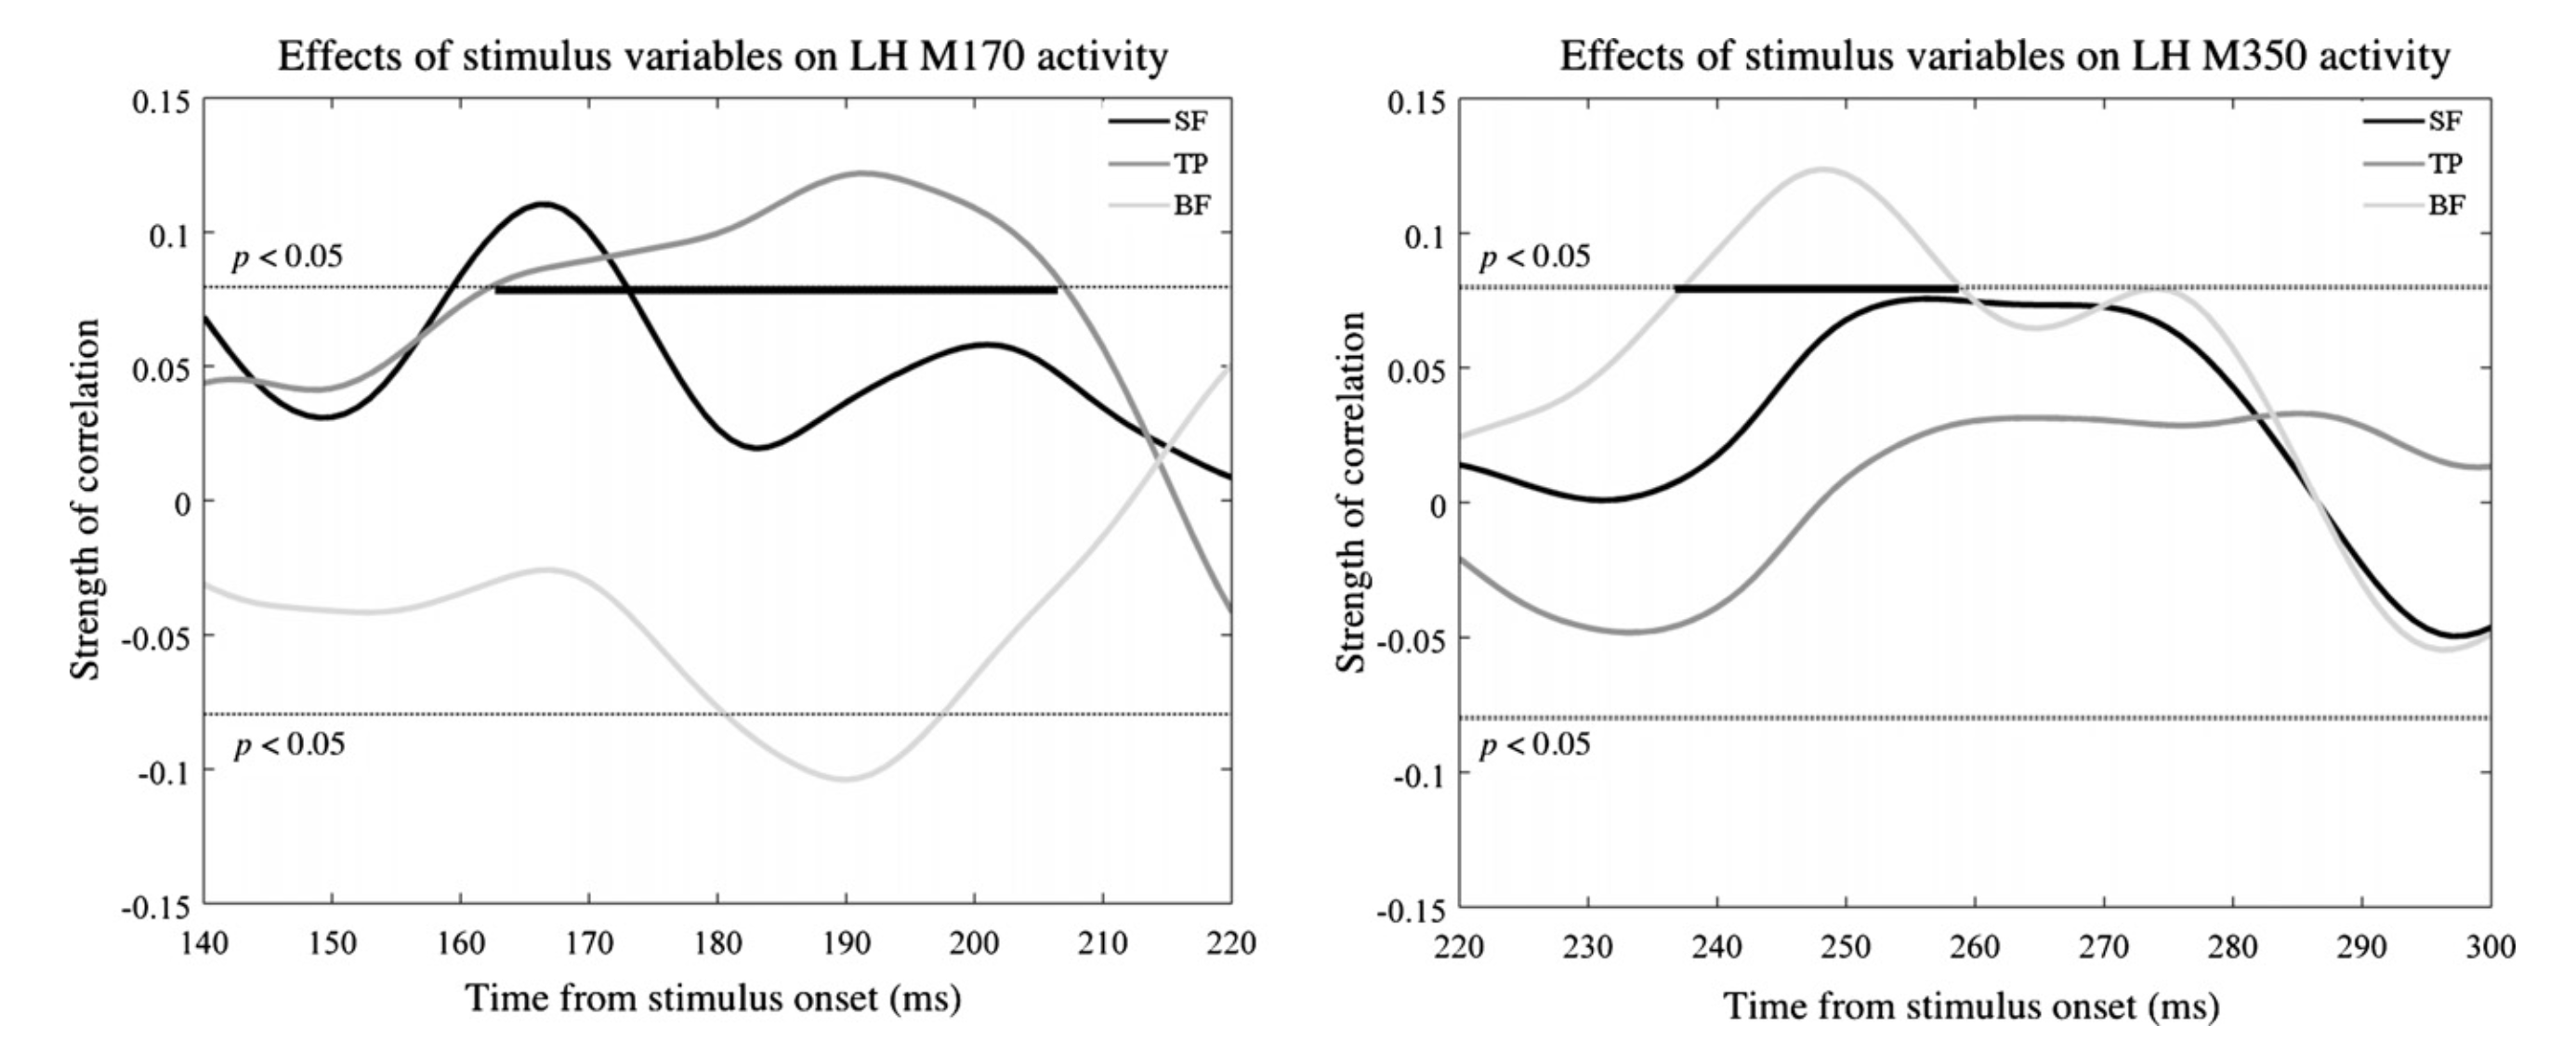
\includegraphics[width=0.99\linewidth]{figs/lewisetal-fig4.png}
\end{center}

\begin{answer}
{
It's tracking not the TP but the surface frequency of the word. In other words, this is a measure of the word in its entirety.
}
\end{answer}

\paragraph{Q2} How is this finding a challenge to the theory of obligatory early decomposition?
\begin{answer}
{
It's inconsistent with the idea that we always decompose a word based on its orthography first. Here it looks like we process the word in its entirety, and \emph{then} decompose it.
}
\end{answer}

% TP: transition probability. TP(formidable) > TP(taxable)

% SF: surface frequency (employer, brother)

% BF: base frequency (employ, employs, employing, employed, broth, broths, \dots{})

% The M170 is associated with TP, about 170ms after seeing the stimulus.

% Here they tested \emph{brother} and \emph{corner} words.


% the pseudo-affixed brother words of the present study yielded a significant effect of surface frequency on amplitude of averaged M170 activity. 


% Full decomposition models could be strengthened if future work confirms that surface frequency effects at the M170 are only present for words like brother for which the decomposition route is completely unmotivated (a true garden path) while always absent for truly affixed words like worker for which decomposition is possible (including those words for which decomposition yields bound roots as in tolerable). In particular, to address theories like that of Hay (2001) that suggest that words with high transition probabilities from stem to suffix (words with high suffix dominance) would be recognized as wholes, rather than through decomposition, further research could confirm a difference in surface frequency effects at the M170 between such words and the pseudo-affixed words, which should be recognized as wholes according to all models under discussion.

% \vfill

\end{document}